
\documentclass[bachelor,german]{hgbthesis}
\RequirePackage[utf8]{inputenc}
\usepackage{amsmath}
\usepackage{stackengine}
\usepackage{graphicx} 
\usepackage{float}

\setlength{\parindent}{0pt}
\graphicspath{{images/}}
\begin{document}
\title{Outlook/Exchange Adapter für CGM G3 Clinical Information System MRP (Multidimensionales Ressourceplanning)}
\author{Krainer Philipp}
\studiengang{Medizin- und Bioinformatik}
\studienort{Hagenberg}
\abgabedatum{2016}{07}{01}	% {YYYY}{MM}{DD}

\nummer{1310458007-B}   % XX...X = Stud-ID, z.B. 0310238045-A  
												%%% (A = 1. Bachelorarbeit)
\gegenstand{Softwareentwicklung mit klassischen Sprachen}                      
\semester{Sommersemester 2016} 
\betreuer{Oliver Krauss}



%\frontmatter
%\pagenumbering{arabic}
%\maketitle

\tableofcontents

%

\mainmatter
\chapter{Einleitung}

\section{Einführung}
Diese Arbeit ist der Praktische Teil der Bachelorarbeit und wurde im Rahmen des Semesterpraktikums verfasst. Das Praktikum im Umfang von 16 Wochen wurde bei der Firma CGM Clinical Austria am Standort Linz absolviert. CompuGroup Medical (CGM) ist der einzige österreichische Softwarehersteller, der umfassende IT-Lösungen zur Optimierung des Gesundheitswesens produziert. Software-Lösungen, welche die Prozesse von niedergelassenen Ärzten und dessen Personal sowie von medizinischem, pflegerischem und administrativem Krankenhauspersonal unterstützen. Die CGM beschäftigt in Österreich 250 Mitarbeiter.

\section{Zielsetzung}
Das Modul MRP errechnet ideale Termine für Operationen in einem Krankenhaus unter der Berücksichtigung aller beteiligter Ressourcen ( Personen ,Geräte, Material) und aller vor und nachgelagerten Untersuchungen sowie Bett und Zimmer. Ziel dieses Projektes ist es für alle ressourcenbezogenen Daten (z.B. Dienste von Ärzten , OP Termin mit spezifischen Ärzten) eine Möglichkeit zu schaffen, Termine in den persönlichen Kalendern der Personen (Teams) anzuzeigen, damit die Anwender in ihrer gewohnten Umgebung die Ergebnisse des komplexen Planungsprozesses vermittelt bekommen. Darüber hinaus wäre eine Darstellung auf mobilen Geräten möglich. Programmiert wird in Java EE und AngularJs.
 
\section{Motivation für die Anwendung der EWS-API}
Grundsätzlich wird davon ausgegangen, dass Termine im Outlook eingetragen werden. Dies sollte automatisch nach der Generierung von vorgegebenen Terminvorschlägen geschehen. Diese Terminvorschläge werden als Teil des MRP-Systems generiert. Die Aufgabe war es mit Hilfe der Java EWS API die Daten an das Outlook zu senden bzw. an den Server zu übermitteln. Die EWS API erleichtert das Arbeiten mit Outlook enorm.\\

Bei relativ flexibler API, kann sowohl Java, C\# als auch  XML verwendet werden. Die Termine werden dabei in Outlook-Kalendern dargestellt. Änderungen von Terminen haben keine Auswirkung auf das MRP System. Weiters können sogenannte "`Appointments"' mit Hilfe von vordefinierten Filtern gesucht und exportiert werden. Dies ermöglicht eine einfachere Handhabung von Abfragen. Die Appointments werden dann in Outlook-Termine umgewandelt und können so exportiert werden. 
\chapter{State of the Art}
Im folgenden Kapitel werden die Features vom MRP-Planungssystem sowie der EWS Schnittstelle dargestellt.

\section{EWS API}
Die Java Exchange Web Services (EWS) Application Programming Interface (API) ist eine Schnittstelle, die von Microsoft bereitgestellt wird, welche die Kommunikation mit einen Microsoft Exchange-Server zulässt. Die API kann mit Java, C\# angesteuert werden und beinhaltet einen umfangreichen Funkionskatalog um die verschiedenen Funktionen in Microsoft Outlook anzusteuern. Diese Funktionen dienen zur Verwaltung von Emails, Kontakten, Aufgaben, Terminen, Kalendern sowie Rechten. Die API wurde entwickelt um programmgesteuerte Abfragen und Aufgaben mit Hilfe eines Microsoft Outlookservers zu realisieren. Sie unterstützt synchrone sowie asynchrone Abfragen und Anfragen an den Server, die zur Abfrage von Verfügbarkeiten und Benutzerrechten sowie von Microsoft Outlookelementen und Ordnern dienen. Weiters kann mit Hilfe der API gefiltert und gesucht werden, weiters lässt die EWS API einen Mehrbenutzerbetrieb zu.\cite{ews2016}
\subsubsection{HyperText Transfer Protocol und HyperText Transfer Protocol Secure}
Das Internetprotokoll HyperText Transfer Protocol (HTTP) beschreibt die zustandslose Übertragung von Internetdaten. Die Übertragung läuft über die Webmethoden GET, PUT und POST. HTTP verwendet die Standardports, welche in der Transmission Control Protocol (TCP)-Richtlinie definiert worden sind.\\ HyperText Transfer Protocol Secure (HTTPS) stellt die sichere Verbindung von HTTP dar, wobei die Verschlüsselung über Secure Socket Layer (SSL) erfolgt. Webseiten werden mittels HyperText Markup Language (HTML), JavaScript und Personal Home Page (PHP) angesteuert, wobei die Daten mit Extensible Markup Language (XML) und JavaScript Object Notation (JSON) übertragen werden.\cite{ews2016,w3c}
\subsection{Funktionen}
\subsubsection{Exchange Service}
Der Exchange Service ist der zentrale Service, welcher Aufgaben verarbeitet und in Verbindung mit dem HTTP(S) Protokoll den Exchange-Server ansteuert. Dieser Service stellt die Verbindung mit dem Server mittels Benutzername, Passwort, Serveradresse her. Außerdem sind zusätzliche Informationen zur Serverversion und Übertragungsart gespeichert. Um die Kommunikation mit dem Server zu ermöglichen, muss die EWS Funktion freigeschaltet sein.\cite{ews2016}
\subsubsection{Items und Folder}
Die Funktionen der EWS API funktionieren nach dem Prinzip der Eindeutigkeit. Dies bedeutet, dass jeder Ordner, jedes Mail und jeder Termin seine eigene ID besitzt, welche vom Server festgelegt wird. Dabei gibt es keine Einschränkung, da jedes Element über die gleiche Priorität verfügt. Weiters kann mit Hilfe dieser eindeutigen ID jedes gesonderte Element abgerufen und beliebig verändert werden. Die Ordner  verfügen über eine eindeutige ID mit der auf den ganzen Ordner zugegriffen werden kann. Auch besitzen spezielle Ordner wie z.B. der Posteingang sogenannte \textit{WellKnownFolderName}s, welche wie Aliase bzw. Pseudonyme für IDs fungieren.\cite{ews2016}
\subsubsection{Email}
Emails können mit Hilfe der API gesendet und empfangen werden. Dabei besitzt jedes Email einen zugeordneten Ordner. Die Emails werden automatisch versendet sobald sie am Server eingetroffen sind. Auch können Emails von beliebigen Konten abgefragt und verändert werden. Vordefinierte Kategorien ermöglichen eine organisierte Verwaltung. Es können Dateien aus dem lokalen Dateisystem an Emails angehängt werden. Wichtige Emails können per Filter gesucht und gefunden werden sowie Posteingangsregeln erstellt und abgerufen werden. Emails können bei Bedarf in einen Unterordner verschoben werden. \cite{joos2013}
\subsubsection{Termine / Appointments}
Termine können erstellt, abgerufen und gelöscht werden. Sie repräsentieren eine Hauptfunktionalität im Outlook. Jeder Termin beinhaltet Datum, Zeit, Ort sowie Teilnehmer. Die Termine werden in den persönlichen Kalendern abgelegt. Weiters können den Terminen optionale Teilnehmer hinzugefügt werden. Periodisch wiederholende Termine werden als Serientermine hinterlegt. Neben dem Hauptkalender können zusätzliche Kalender erstellt werden. Eine weitere Funktionalität stellt die Abfrage von Verfügbarkeiten dar. Diese liefern in weiterer Folge Terminvorschläge. Dabei wird auch die terminliche sowie räumliche Verfügbarkeit mitgeliefert. \cite{joos2013}

\subsubsection{Tasks}
Ein weitere Funktionalität der API stellen Tasks dar, welche erstellt und abgerufen werden können. Tasks enthalten eine Liste von Aufgaben, welche Personen zugeordnet werden und von diesen abgearbeitet werden. Einzelne Aufgaben können priorisiert und kategorisiert werden.\cite{ews2016}
\subsubsection{Kontakte}
Kontakte stellen neben den Terminen eine wichtige Rolle in der Microsoft Outlookumgebung dar. Die Kontakte werden im Adressbuch verwaltet und können angelegt, abgerufen sowie gelöscht werden. Kontakte können aus vordefinierten Dateien importiert und exportiert werden. Das Adressbuch enthält Kontakte sowie Kontaktgruppen. In den Kontakten sind Namen, Telefonnummern, Emailadressen und persönliche Daten hinterlegt. In dem Adressbuch kann gesucht und gefiltert werden.\cite{joos2013}

\section{Multidimensionales Ressourcen Planning (MRP)}

Das MRP-System ist zur Planung von Krankenhausterminen entwickelt worden. Die Hauptaufgabe von MRP ist es aus gegebenen Ressourcen (Personen, Räume, Geräte, Betten, Materialien) in Verbindung mit Regeln Planungskalender für einzelne Räume zu erstellen. Diese Kalender repräsentieren Operationsplanungen, die eine zentrale Einheit in einem Krankenhausinformationssystem (KIS) darstellen.\\ Ein KIS besteht in erster Linie aus den Zentralkomponenten Organisation, Bettenmanagement, Aufnahme, Entlassung sowie Operationsplanungen. MRP deckt nicht die zentralen Komponenten ab, da sich dieses System nur mit der Planung von Räumen und Terminen mithilfe von Ressourcen beschäftigt. Es übernimmt nicht die Verwaltung des Krankenhauses! \cite{g3mrp,haas2004}
\subsection{Funktionsweise}
Das MRP System generiert aus vorgegebenen Daten geeignete Termine und Pläne für Räume des Krankenhauses. Es werden die benötigten Ressourcen gesammelt und in einer zentralen Datenbank  verwaltet. Aus den Datensätzen werden mittels Ressourcenmanager die Ressourcen zusammengetragen und Appointments generiert. Diese werden dann mit Hilfe des Kapazitätsmanagementtools den verfügbaren Kapazitäten der einzelne Ressourcen zugeordnet und in einer Kalenderansicht dargestellt. \cite{g3mrp}\\
\subsection{Masterdata}
Jedes Feature im MRP-System folgt der selben Struktur. Jedes Feature besteht aus den Teilen API, Component, Datenbank und Service. Dabei wird die Drei-Schichten-Architektur realisiert. Dies bedeutet, dass es drei getrennte Implementierungen hinsichtlich jeder Schicht gibt, welche als eigenständig fungieren. Die unterste Schicht wird als Datenbank-Schicht bezeichnet und ist zuständig für die Verwaltung von persistenten Daten. Die Mittlere Schicht wird als Business-Logik bzw. Verarbeitungsschicht bezeichnet. Diese ruft die Daten von der untersten Schicht ab und leitet sie gegebenenfalls an die oberste Schicht weiter. Es besteht die Möglichkeit für Berechungen und Änderungen der Daten. Die oberste Schicht stellt die Präsentationsschicht dar und ist zuständig für die visuelle Darstellung der Daten. Die 3-Schichten-Architektur hat den Vorteil, dass die Aufgaben der Schichten klar von einander getrennt sind. Weiters gibt es die Component-Service-Implementation, welche aus den Komponenten, Datenbank, Service, und API besteht.\cite{g3r,g3mrp}
\subsubsection{Struktur}
Jedes Feature folgt der Component-Service-Implementation, welche aus folgenden Teilen besteht(siehe Abb. 2.1)\cite{html5,g3r,g3rp,g3mrp}:\\
	\begin{figure}[H]
	\centering
		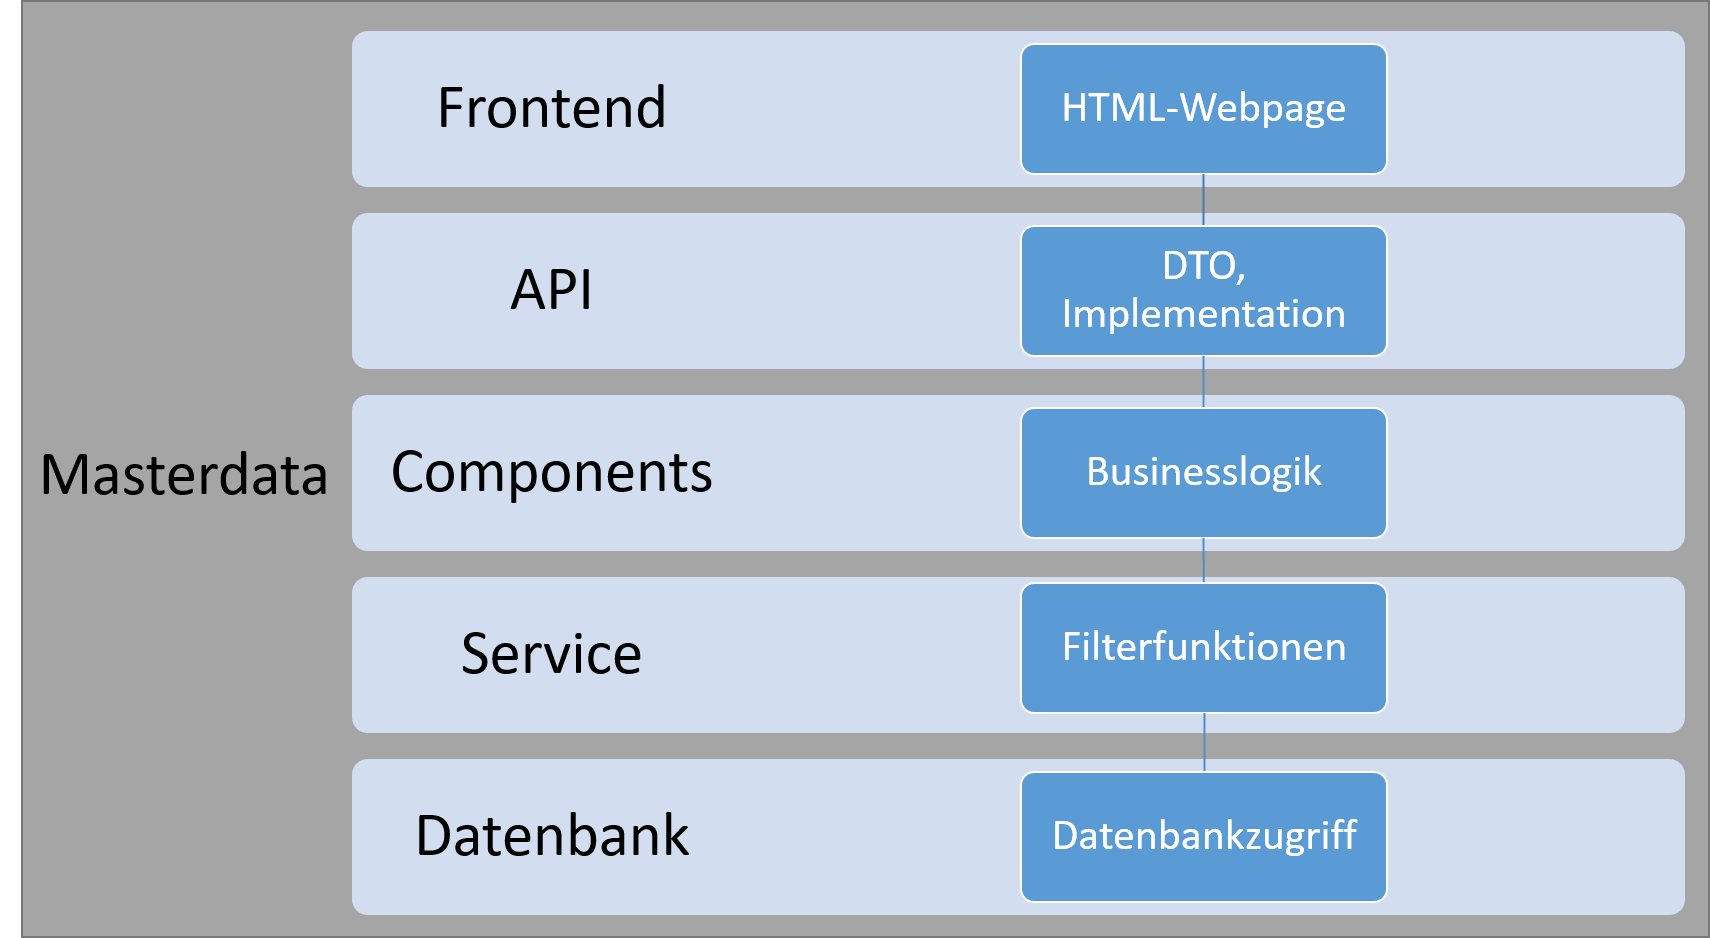
\includegraphics[width=0.8\textwidth]{diagramm1.png}
\caption{Architekturdiagramm}
\end{figure}

 \begin{itemize}
	


\item \textit {Datenbank:} Das Datenbankfeature verwaltet alle Daten in einer Datenbanktechnologie, welche variabel auswählbar ist. Das Speichern und Abrufen von Daten wird über den jeweiligen Datenbanktreiber betrieben, welcher mit einer standardisierten Datenbankansteuerung kommuniziert. Dieser befindet sich innerhalb eines Data Access Object (DAO). Dieses beinhaltet die relevanten Datenbankzugriffsfunktionen und liefert ein Data Transfer Object (DTO).\\
\item \textit{Service:} Der Service erhält Daten von der Datenbank und schickt sie an die Components weiter. Die Services dienen den Components für eine erleichterte Abfragemöglichkeit von Datenobjekten. Weiters benötigen die Services vordefinierte Filterfunktionen. Die Funktionalität der Services gehört der Business-Logik-Schicht an.\\
\item \textit{Components:} Die Components stellen im Feature die Hauptbestandteile dar und sind ein Teil der Businesslogik. Die Components repräsentieren die eigentliche Logik, da in diesen Funktionen die Verarbeitung der Daten erfolgt. Die Components erhalten die Daten aus der Datenbank und wandeln diese in \textit{Data Transfer Objects} um. Die Objekte werden an die API weitergeleitet.\\
\item \textit{API:} Die API ist ein Teil der Businessschicht und stellt die Verbindung zum Frontend da. Die API bekommt die Daten von den Components und wandelt diese in webkonforme Übertragungsobjekte um, welche an das Frontend weitergeleitet werden. Außerdem ist die API zuständig für das Empfangen von Daten aus dem Frontend.\\
\item \textit{Frontend:} Das Frontend repräsentiert die Präsentationssschicht, welche für den jeweiligen Benutzer sichtbar ist. Im Frontend werden die Benutzerinteraktionen verwaltet, Daten zu Transferobjekte umgewandelt und an das Backend gesendet. \\
\item \subsection{Hospital Information System}
Das Hospital Information System (HIS) von CGM wird unter der Produktbezeichnung G3 HIS geführt und besteht aus mehreren Modulen. Die Zentralkomponenten eines KIS sind in diesem System integriert und bilden eine einheitliche Weboberfläche. Diese ist betriebssystemunabhängig und wird in einem vom G3 HIS unterstützten Browser verwendet. Das G3 HIS Projekt umfasst mehrere Projektgruppen, die in die unterschiedlichen Aufgaben (Organisation, Bettenmanagement, Aufnahme, Entlassung, Operationsplanungen) eines Krankenhauses unterteilt sind. Sie bieten eine umfangreiche Konfiguration und Verwaltung der einzelnen Funktionsgruppen bzw. Module an. Die Software stellt die 3. Generation dar und wird ständig weiterentwickelt.
\end{itemize}











\chapter{Konzept und Design}
In diesem Kapitel wird das Konzept zur Übertragung von Daten aus dem MRP ins Microsoft Outlook beschrieben. 


\section{Ansteuerung mittels MRP}
MRP ist eine von CGM entwickelte Software, die Termine für Operationen in Krankenhäusern unter der Berücksichtigung aller beteiligter Ressourcen optimiert und berechnet. Das MRP-Modul beinhaltet folgende Funktionalitäten\cite{html5,g3r,g3mrp}:\\
\begin{enumerate}
	\item Zu Beginn werden die verfügbaren Ressourcen (Personen, Räume, Geräte, Betten, Materialien) angelegt und zugeordnet.  
	\item Zuordnung der ressourcenbezogenen Daten: Jeder  Ressource werden Informationen zugeteilt.
	\item Mittels der Ressourcen werden mithilfe von Kapazitäten(terminliche Verfügbarkeiten) Organisationseinheiten (Zeitbereiche mit verknüpften Ressourcen) gebildet.
	\item Aus diesen Einheiten werden Vorschläge gebildet. Diese Vorschläge beinhalten lediglich eine Zeitspanne. Um einen Termin festlegen zu können, müssen Ressourcen  definiert werden. Dies entsteht aus den bereits hinterlegten Personendaten sowie aus den Verfügbarkeitsabfragen der EWS Schnittstelle. Mit diesen erweiterten Funktionen können konkrete Termine generiert u. nach deren Bestätigung ins Outlook exportiert werden. Die exportierten Termine können im betreffenden Kalender eingesehen werden. Das Anlegen von Ressourcen u. das Selektieren von exportierten Terminen erfolgt manuell.\\
\end{enumerate}	

Die Erstellung eines MRP Moduls erfolgt nach den Programmierrichtlinien von CGM. Dieses Modul dient zum Export von generierten Terminen ins Outlook. Weiters werden Filter- und Suchfunktionen bereitgestellt. Diese können MRP-Appointments und Outlook-Appointments filtern und suchen.





\chapter{Implementierung}
In Abstimmung mit CGM wurde das Konzept aus Kapitel 3 für die Umsetzung gemäß Zielsetzung herangezogen. Dabei wurden die Funktionen der EWS-API verwendet und in den Methoden der nachfolgenden Module aufgerufen: 
\section{Microsoft Outlook}
Die nachfolgenden aufgelisteten Packages beziehen sich auf die Klassen: 
	 \textit{Packagename + Service },
	 \textit{I + Packagename + Service} und
	\textit{Packagename + Dto} (siehe Klassendiagramm Abb. 4.1)

Die jeweilige Klasse des Packages implementiert eine vordefinierte Schnittstelle (Interface), welche einen vordefinierten Benennungsschema folgt. Die Funktionalitäten sind unabhängig vom MRP-System, können aber von diesem verwendet werden. Die für die Arbeit entwickelten Datentypen sind im Package \textit{Model} definiert. Diese Klassen können gleichnamige Klassen im MRP haben, haben aber keine Beziehung zu diesen Klassen. \\


	\begin{figure}[H]
	\centering
\noindent\makebox[\textwidth]{%
		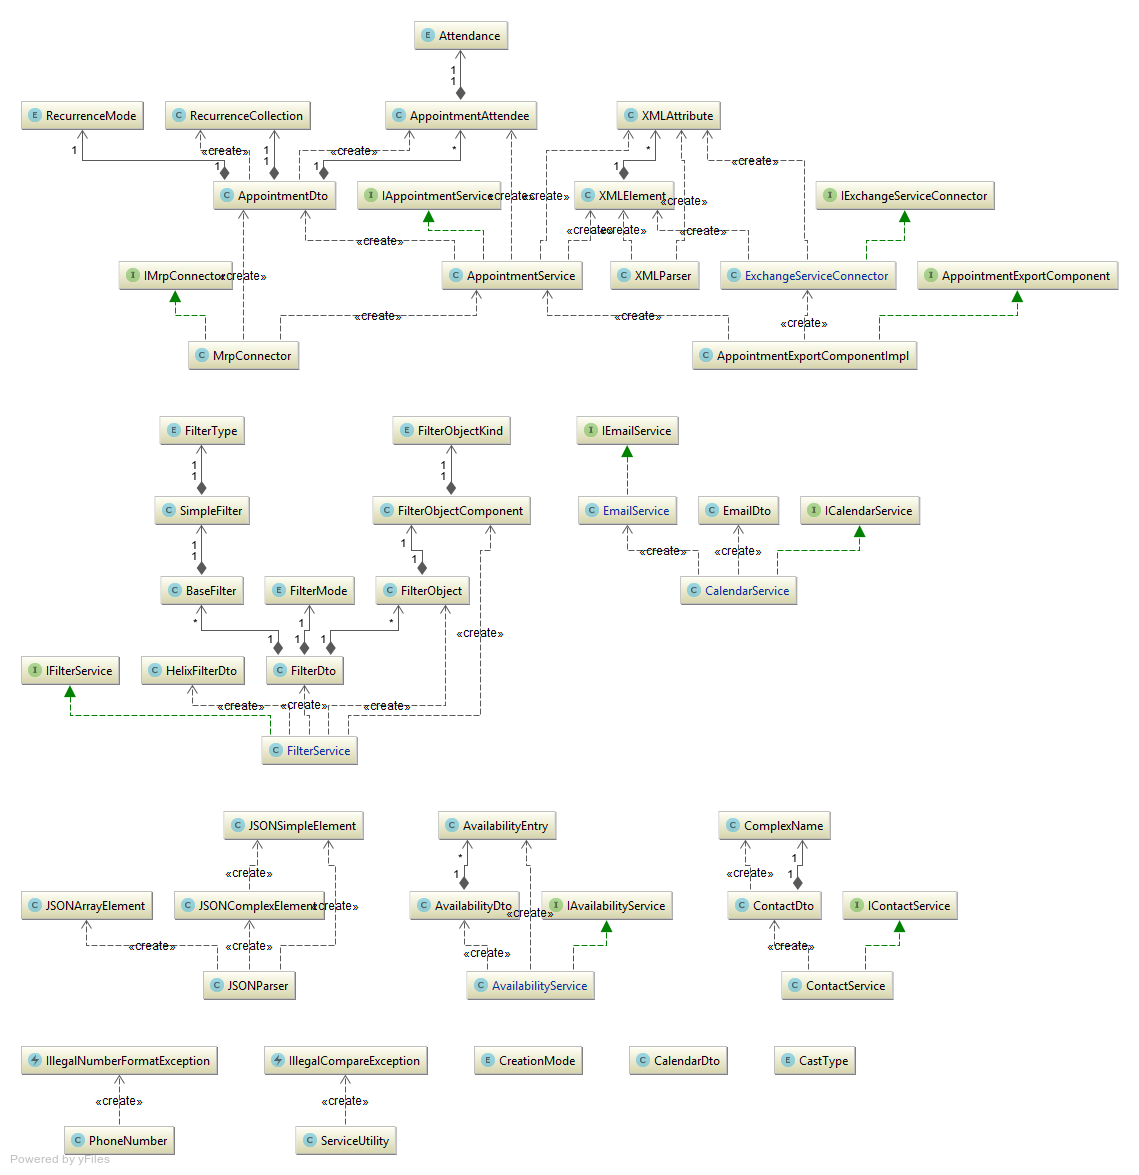
\includegraphics[width=1.2\textwidth]{diagram.png}}
\caption{Klassendiagramm}
\end{figure}


\subsection{Exchangeservice}
Der Exchangeservice dient als zentrale Verbindung zum Microsoft Outlook. Die Features bzw. Methoden, welche mit dem Exchange-Server kommunizieren, verwenden ExchangeService als Parameter. Die Klasse wird \textit{ExchangeServiceConnector} genannt und ist zuständig für die Verbindung zum Server sowie für die Anfragen der Features. Dieser Service bezieht sich ausschließlich auf das eigene Outlookkonto bzw. auf das Konto, welches mit Passwort und Benutzername angegeben wird. Weiters besteht die Möglichkeit die Exchangeserverversion festzulegen. Diese Klasse implementiert das zugehörige Interface \textit{IExchangeServiceConnector}.\\ Die Serververbindung wird mit Hilfe der Methode \textit{createServerConnection} initialisiert, wobei der Benutzername und das Passwort als Parameter übergeben werden. Die gleichnamige Methode verwendet zusätzlich den Parameter Server-URL. Die Methode \textit{createServerConnection} baut mit Hilfe der Daten eines XML-Dokuments eine Serververbindung auf. Die genanten Methoden retournieren eine Instanz des Exchangeservice. Dieser Service existiert nur einmal zur Laufzeit. Damit wird garantiert, dass immer der gleiche Server angesteuert wird. Mit der Methode \textit{saveSettingsToXML} können die Servereinstellungen in einem XML-Dokument gespeichert werden. 
\subsection{Model}
Die verwendeten Objekte bzw. Datentypen in den einzelnen Features bzw. Packages werden im Model repräsentiert. Die einzelnen Klassen repräsentieren die jeweiligen Datentypen, welche einer vordefinierten Struktur folgen. Diese folgt der Bean-Definition. Diese bedeutet, dass alle Membervariablen \textit{private} sind und daher wird auf die Variablen mit Getter und Setter zugegriffen. Die einzelnen definierten Datentypen besitzen einen öffentlichen Default-Konstruktor ohne Parameter.
\subsection{Kalender}
Mittels Kalenderservice können Kalender angelegt und abgerufen werden. Der \textit{CalendarService} implementiert das zugehörige Interface \textit{ICalendarService} und verwendet den Datentyp \textit{CalendarDto}.\\ Die Mehode \textit{getCalendars} ruft die verfügbaren Kalender einer Emailadresse ab. Die Emailadresse repräsentiert Personen oder Räume. Zusätzliche Kalender werden durch die Methode \textit{createNewCalendar} angelegt. Auch gibt es die Methode \textit{sendWarningToUser}, mit dieser kann ein Email an den betreffenden Benutzer versendet werden. Die Emailnachricht enthält die betreffende Warnung.
\subsection{Appointments}
Mit Hilfe des Appointmentservices können Microsoft Outlook-konforme Appointments angelegt, verwaltet und abgerufen werden. Weiters ist möglich Appointments in einem XML-Dokument zu speichern. Das XML Dokument beinhaltet die Datenfelder aus dem \textit{Model} in einer validen XML-Struktur. Diese XML-Dokumente können zur Erstellung von Appointments verwendet werden. Es besteht die Möglichkeit Konflikte zu betreffenden Appointments vom Server abzufragen. Der \textit{AppointmentService} implementiert das zugehörige Interface \textit{IAppointmentService} und verwendet den Datentyp \textit{AppointmentDto}. \\ Mit der Methode \textit{createAppointment} kann ein Appointment angelegt werden. Der \textit{ExchangeService} wird als Parameter übergeben. Die Methode \textit{buildAppointment} erstellt den Datentyp \textit{Appointment}. Die Methode \textit{createAppointments} ermöglicht das gleichzeitige Speichern und Anlegen von Appointments. Eine weitere Funktionalität ist durch die Methode \textit{hasConflictedAppoinments} gegeben. Diese Funktion überprüft mit Hilfe des Exchangeservers Konflikte bei betreffenden Appointments. Die Funktionen \textit{appointmentListToXML}, \textit{xmlToDto} und \textit{xmlToAppointmentList} ermöglichen die Verwaltung von outlookkonformen Appointments mithilfe von XML.
\subsection{Availability}
Durch den Availabilityservice können Verfügbarkeiten von Personen und Räumen abgefragt werden. Der \textit{AvailabilityService} implementiert das zugehörige Interface \textit{IAvailabilityService} und verwendet den Datentyp \textit{AvailabilityDto}. \\ Die Hauptfunktion \textit{checkAvailability} ruft mit Hilfe des \textit{ExchangeService} Verfügbarkeiten über die EWS-Schnittstelle ab. Die Methode \textit{checkAvailbilityForPerson} überprüft die Verfügbarkeit von  Personen anhand deren Email-Adressen. Mit Hilfe der Methode \textit{checkAvailbilityForRooms} können im Gegensatz zur obengenannten Methode anstelle von Personen Räume abgefragt werden. Die beiden Funktionen \textit{getRoom} und \textit{getAllRooms} liefern Räume zurück.  Personen und Räume werden durch die jeweiligen Emails repräsentiert.
\subsection{Kontakt}
Der Kontaktservice ermöglicht das Anlegen, Abrufen und Verwalten von Outlookkontakten in den jeweiligen persönlichen Adressbüchern. Der Kontaktservice arbeitet mit dem Benutzer des Exchangeservices. Der \textit{ContactService} implementiert das zugehörige Interface \textit{IContactService} und verwendet den Datentyp \textit{ContactDto}.\\ Die Methode \textit{getContacts} ruft persönliche Kontakte des angemeldeten Benutzers aus dem persönlichen globalen Adressbuch ab. Die Kontakte sind unsortiert und können mittels Filter zusätzlich gefiltert werden. Neue Kontakte werden über die Funktion \textit{buildContact} erstellt. Die Funktion \textit{getContactDtos} liefert mithilfe der Funktion \textit{buildContact} eine Liste vom vordefinierten Datentyp \textit{ContactDto}. 
\subsection{Email}
Der Emailservice ermöglicht das Senden von bestehenden Emails. Diese beinhalten die relevanten Felder der Emails. Weiters können die Emails aus dem jeweiligen Postfach des Benutzers aufgerufen werden. Der \textit{EmailService} implementiert das zugehörige Interface \textit{IEmailService} und verwendet den Datentyp \textit{EmailDto}.\\ Durch die Mehode \textit{sendEmail} können Emails versendet werden. Diese werden in der Mehode \textit{buildEmail} erstellt und enthalten alle relevanten Informationen zu Sender und Empfänger sowie Betreff und Emailtext. Die Methode \textit{getEmails} ruft eine vordefinierte Anzahl Emails aus dem Posteingang ab. 
\subsection{Filter}
Die Filter bestehen aus Filterkomponenten, welche vordefiniert sind. Diese Filterkomponenten folgen dem Prinzip der überpersistenten Speicherung. Dies bedeutet, dass bereits gefilterte Daten trotzdem erhalten bleiben. Grundsätzlich ist jede Filterkomponente aus zwei Teilen aufgebaut: Der erste Teil beinhaltet die Informationen zu den Filtern. Der zweite Teil stellt eine Datensammlung dar. Diese Daten bleiben solange erhalten solange die Filterkomponenten aktiv sind. Die Filterkomponenten werden gleichzeitig bzw. hintereinander angewendet, um die logischen Funktionen AND und OR zu repräsentieren Eine weitere Funktionalität ist der Vergleich von Methoden mit den Variablen.\\ Die Mehode \textit{apply} beschreibt die Hauptfunktionalität des Filters und beinhaltet die Funktionalität, die zur Anwendung eines bestimmten Filters erforderlich ist. Das \textit{FilterDto} beinhaltet sowohl die Filterkomponenten als auch die zu filternden Daten. Mit der Methode \textit{applySimpleFilter} wird ein Filter für eine Sammlung von zu filternden Objekten angewandt. Die Funktion \textit{applyFilter} wird verwendet, wenn die zu filternden Objekte den Typ \textit{AppointmentComponent} darstellen. Die zwei Funktionen \textit{applyHelixFilter} werden verwendet, wenn die Filter vom MRP-System stammen. Die Funktionen \textit{getFiltered} und \textit{getUnfiltered} dienen zum Abrufen von gefilterten und ungefilterten Daten eines \textit{FilterDto}s

\section{Masterdata-Feature}
Als Masterdata werden Features bezeichnet, welche zentrale Daten im MRP verwalten und welche in einer Datenbank gespeichert werden (siehe Abb. 4.2).
\begin{sidewaysfigure}
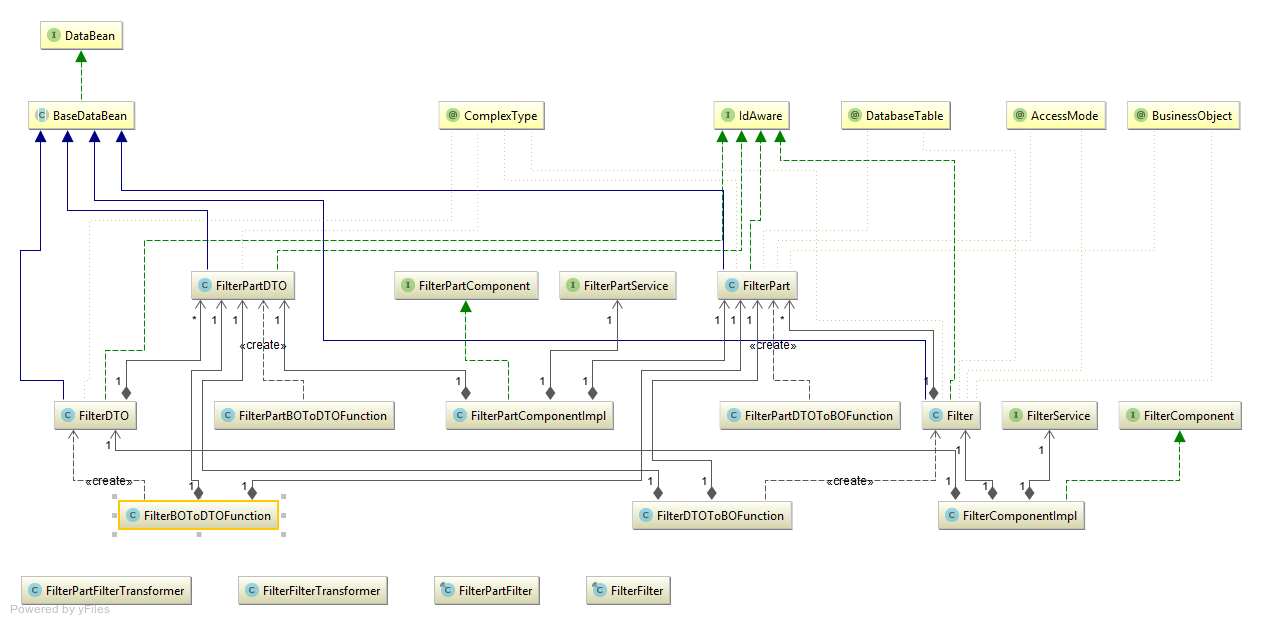
\includegraphics[width=\textheight]{diagrammrp.png}
\caption[]{Klassendiagramm}
\end{sidewaysfigure}

\subsection{Filter}
In dem MRP-Feature Masterdata wurde ein Feature hinzugefügt, welches zur Verwaltung von Filtern dient. Die Filter werden in der zentralen Datenbank von MRP gespeichert und über die Weboberfläche von MRP verwaltet, da die Filter zu den Masterdata-Features zählen. Die Filter dienen zur Filterung von MRP-Appointments. Jeder Filter beinhaltet die benötigten Filterkomponenten, welche für das Filtern der Daten verantwortlich sind. 
\subsection{Filterkomponenten}
Jeder Filter hat Filterkomponenten untergeordnet, welche die Informationen zu Filterart, Filtertyp und Filterwert enthalten. Diese Komponenten werden in einer Relation zu den Filtern in der Datenbank abgelegt. Die Filterkomponenten sind immer für einen bestimmten Filter zuständig und können nicht einzeln verwendet werden. Diese Filterkomponenten dienen zum Filtern von Appointments.
\subsection{Weboberfläche}
In der Weboberfläche von dem MRP-System werden die Filter und Filterkomponenten verwaltet. Die Oberfläche wird von G3 HIS bereitgestellt und bietet die Funktonalität von MRP. Mit Hilfe der Filter werden Appointments gesucht und angezeigt. Zukünftig sollen selektierte Appointments ins Microsoft Outlook exportiert werden können.



 

\chapter{Evaluierung}
\section{Einleitung}
Das Outlookmodul ist im MRP-System teilintegriert. Die Testumgebung wird mit Hilfe eines Jenkins-Maven-Testserver realisiert, welcher selbständiges automatisiertes Testen zulässt. Bei einen Jenkins-Maven-Testserver handelt es sich um einen Linux-Server, welcher das gesamte Projekt in regelmäßigen Abständen compiliert und die vorgesehenen Tests ausführt. Die Ergebnisse sind in einer Weboberfläche einsehbar. In dem Repository gibt es die Branches \textit{master} und \textit{dev}. Diese werden in die automatisierte Testumgebung integriert und in fixierten Zeitabständen getestet. Da das zu bearbeitende Modul kein Teil der zwei Branches ist, kann es nicht getestet werden. Durch den Umstand des Testprozesses muss auf andere Testmittel umgestiegen werden.

\section{Benutzerinteraktives Testen}
Auf Grund des Testprozesses wird auf die Methodik benutzerinteraktives Testen zurückgegriffen. 
Die gewählte Methodik ist besser bekannt als \textit{Whitebox-Test}.\cite{SpillnerLinz05} Diese Methodik beruht auf der visuellen Kontrolle des Programmierers. Dabei überprüft der Programmierer die Ergebnisse in der grafischen Oberfläche bzw. Konsole. Die Testmethodik dient rein zur visuellen Kontrolle ob die geforderten Datenfelder richtig in der Konsole angezeigt werden. Trotzdem kann mit Hilfe dieser Methodik die Funktion des Programms getestet werden. Dies ist auch möglich wenn kein geeignetes Testframework vorhanden ist. Da das Modul mit einem Server  kommuniziert, bei dem die Verarbeitung der Anfragen einen Engpass darstellt, stellt sich automatisiertes Testen mittels Frameworks als aufwendig und komplex dar. 
\newpage
Im Rahmen der Testung werden folgende Funktionen überprüft:\\

\begin{table}[H]
\centering
\begin{tabular}{|l|c|}
\hline
Getestete Funktionen&Tests erfolgreich\\ \hline
Appointments anlegen& 16\\ \hline
Appointments abrufen& 24\\ \hline
Availablilities abfragen&20\\ \hline
Kalender anlegen&21\\ \hline
Kalender abfragen&21\\ \hline
Kontakte abrufen&14\\ \hline
Adressbuch abfragen&30\\ \hline
Emails senden     &40\\ \hline
Emails abrufen     &45\\ \hline
Serververbindung initialisieren& 5\\ \hline
Serververbindung speichern & 5 \\ \hline
Serververbindung abfragen     &    10    \\ \hline

Filter verwalten     &       38 \\ \hline
Filterkomponenten verwalten     &    64    \\ \hline
Filterkomponenten zuordnen     &    23    \\ \hline
MRP-Filter verwalten     &   12     \\ \hline
MRP-Filterkomponenten verwalten     &       17 \\ \hline
MRP-Appointments exportieren & 0 (keine Tests vorhanden) \\ \hline
\end{tabular}
\caption{Tests}
\end{table}


\chapter {Zusammenfassung}
In diesem Kapitel werden die Ergebnisse zusammengefasst und diskutiert.
\section{Resultate}
Bei dieser Arbeit wurde ein Programm implementiert, welches als Modul für das MRP-System der Firma CGM fungiert. Die Implementierung wurde mittels JAVA durchgeführt. Es wurde die Java EWS API verwendet. Die EWS API dient zur Ansteuerung eines Microsoft Outlookservers mithilfe von Programmmethoden. Das Modul verwendete diese API um bereitgestellte Termine aus dem MRP-System an das Microsoft Outlook zu exportieren. Die Daten wurden von weiteren Modulen des MRP-Systems generiert und bereitgestellt. Allerdings fehlte die Integration des Moduls in das gesamtheitliche MRP-System, da dieses zum damaligen Zeitpunkt noch nicht fertiggestellt war. Das Testen erfolgte durch benutzerinteraktives Testen. Dieses beruhte auf einer rein visuellen Betrachtung des Benutzers. Die diesbezüglichen Tests verliefen positiv.
\section{Diskussion}
Das in dieser Arbeit erstellte Programmmodul ist universell einsetzbar, wurde aber geringfügig an das MRP-System angepasst. Die EWS API mit ihren komplexen Datentypen wurden durch das vereinfachte DTO ersetzt. Die universelle Einsetzbarkeit wurde damit ermöglicht. Die Implementierung der verwendeten Filter wurde generisch gehalten, um eine universelle Einsetzbarkeit zu ermöglichen.


\chapter{Anhang}
\section{Literatur}
\begin{itemize}[label={}]
\setlength\itemsep{1em}
	\item Das Handbuch Microsoft Outlook 2013, Thomas Joos, 2013, O’Reilly Verlag GmbH
  \item JAVA EWS Reference Dokument in GIT, https://github.com/OfficeDev/ews-java-api/wiki/Getting-Started-Guide
  \item CGM G3 HIS Documentation , CGM, Internes Dokument(vertraulich)
	\item G3 Reverse Proxy, 
	\item CGM HTML5 Controls Browser
\end{itemize}



\end{document}